\documentclass[11pt,a4paper]{article}

\usepackage{../../templates/style}

\begin{document}

\begin{problem}{Wheel}{standard input}{standard output}{1 second}{16 megabytes}

ในเกมวงล้อรางวัล มีล้อกลมที่แบ่งเป็น $N$ ช่อง ไล่จากช่องที่ $1$ ไปจนถึงช่องที่ $N$ ตามเข็มนาฬิกา โดยช่องที่ $N$ จะติดกับช่องที่ $1$ ในแต่ละช่องของวงล้อมีรางวัลมูลค่าต่าง ๆระบุไว้ โดยช่องที่ $i$ สำหรับ $1 \leq i \leq N$ จะมีรางวัลมูลค่า $A_i$ บาท วงล้อดังกล่าวหมุนได้ และมีลูกศรชี้ช่องรางวัลปัจจุบันไว้ โดยเมื่อเริ่มต้นลูกศรชี้ช่องที่ $1$ (ดูรูปด้านล่าง)

\begin{figure}[h]
\centering
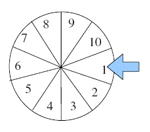
\includegraphics[width=0.4\textwidth]{../latex/img/1055/1055-1.png}
\end{figure}

มีผู้เล่น $K$ คนเข้าร่วมเล่นเกมครั้งนี้ เกมจะดำเนินเป็นตา โดยเริ่มจากผู้เล่นคนที่ $1$ คนที่ $2$ ไปจนถึงผู้เล่นคนที่ $K$ จากนั้น จะวนกลับมาผู้เล่นคนที่ $1$ อีกครั้ง ในการเล่นแต่ละตา ผู้เล่นคนที่เล่นตานั้นจะโยนลูกเต๋า เมื่อได้ผลลัพธ์จากลูกเต๋าแล้วสมมติได้คะแนนเป็น $X$ จะหมุนวงล้อไปในทิศทางทวนเข็มนาฬิกาโดยจะหมุนข้ามช่องที่ยังมีรางวัลอยู่ไป $X$ ช่อง และไปหยุดอยู่ที่ช่องที่มีรางวัลช่องถัดไป ผู้เล่นที่โยนลูกเต๋าจะได้ของรางวัลในช่องนั้น และผลัดให้ผู้เล่นคนถัดไปโยนลูกเต๋า เกมจะดำเนินไปเรื่อย ๆ จนกระทั่งของรางวัลหมด

พิจารณาการเล่นเกมบนวงล้อที่แบ่งเป็น $5$ ช่อง โดยที่มูลค่าของรางวัลในช่องต่าง ๆเริ่มจากช่องที่ $1$ คือ $3, 5, 2, 4$, และ $1$ บาท สมมติว่ามีผู้เล่น $3$ คน ตัวอย่างการเล่นเกมแสดงดังตารางด้านล่าง (หมายเลขช่องที่หมุนข้ามที่แสดงในวงเล็บแสดงช่องในวงล้อที่ไม่มีรางวัลแล้วดังนั้น ในการหมุนให้หมุนข้ามไปเลย)

\begin{center}
		\begin{tabular}{|c|c|c|c|c|c|}
\hline
\textbf{ตาที่}	& \textbf{ผู้เล่น}& \textbf{โยนลูกเต๋าได้}&	\textbf{หมุนเข้าช่อง} & \textbf{หยุดที่ช่อง}	& \textbf{มูลค่าที่ได้}\\
\hline \hline
1	&1	&3	&1,2,3	&4	&4\\
\hline
2	&2&	5	&(4),5,1,2,3,(4),5	&1	&3\\
\hline
3	&3	&1	&(1),2	&3	&2\\
\hline
4	&1	&2	&(3),(4),5,(1),2,(3),(4)	&5	&1\\
\hline
5	&2	&1	&วนสองรอบ	&2	&5\\
\hline
\end{tabular}
\end{center}

ดังนั้น ผู้เล่นคนแรกจะได้รางวัลมูลค่ารวม $5$ บาท คนที่สองมูลค่ารวม $8$ บาท และคนที่สามมูลค่ารวม $2$ บาท

\bigskip
\underline{\textbf{โจทย์}}  ให้เขียนโปรแกรมที่รับข้อมูลของรางวัลบนล้อ และแต้มของลูกเต๋าที่ผู้เล่นแต่ละคนโยนได้ จากนั้นคำนวณว่าผู้เล่นแต่ละคนจะได้รับรางวัลมูลค่ารวมกี่บาท

\InputFile

\textbf{บรรทัดแรก} ระบุจำานวนเต็ม $N$ และ $K$ $(1 \leq N \leq 100; 1 \leq K \leq 20)$

\textbf{บรรทัดที่ $2$ ถึง $N+1$} ในบรรทัดที่ $i + 1$ สำหรับ $1 \leq i \leq N$ จะระบุค่า $A_i$ มูลค่าของรางวัลในช่องต่าง ๆ $(1 \leq A_i \leq 100)$ 

\textbf{บรรทัดที่ $N+2$ ถึง $N+1$} ในบรรทัดที่ $N + j +1$ สำหรับ $1 \leq j \leq N$ จะระบุจำนวนเต็ม $X_j$ แทนแต้มของลูกเต๋าในการโยนครั้งที่ $j$ แต้มของลูกเต๋าจะมีค่าที่เป็นไปได้ตั้งแต่ $1$ ถึง $6$ $(1 \leq X_j \leq 6)$

\OutputFile

\textbf{มี $K$ บรรทัด} แต่ละบรรทัดมีจำนวนเต็มหนึ่งจำนวน ระบุมูลค่ารวมของรางวัลที่ผู้เล่นแต่ละคนจะได้รับ เริ่มจากคนที่ $1$ ถึงคนที่ $K$ กล่าวคือ บรรทัดที่ $i$ ให้ระบุค่ารางวัลของตนที $i$

\Examples

\begin{example}
\exmp{5 3
3
5
2
4
1
3
5
1
2
1}{5
8
2}%
\end{example}


\Source

Young Thai Online Programming Competition 2008

\end{problem}

\end{document}